\chapter{Psalm 46}

\begin{figure}
  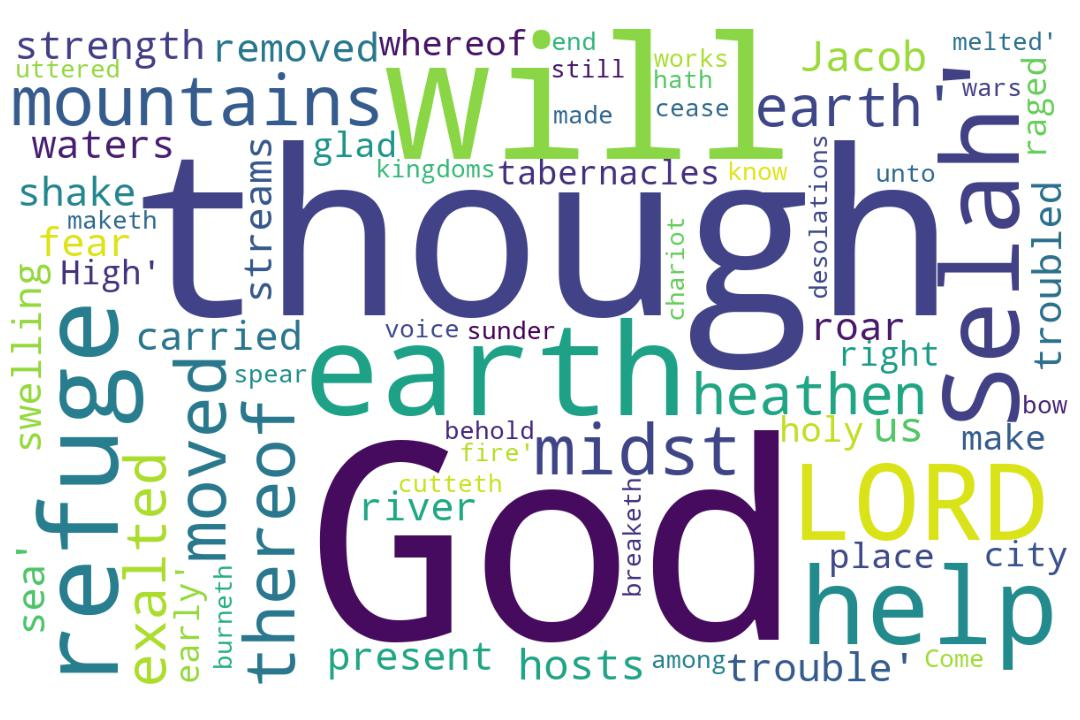
\includegraphics[width=\linewidth]{19OT-Psalms/Psalm46-WordCloud.jpg}
  \caption{Psalm 46 Word Cloud}
  \label{fig:Psalm 46 word Cloud}
\end{figure}

\marginpar{\scriptsize \centering \fcolorbox{bone}{lime}{\textbf{THERE IS A REFUGE}}\\ (Psalm 46) 
\begin{compactenum}[I.][8]
	\item There is a \textbf{Refuge} \index[scripture]{Psalms!Psa 046:01}\index[scripture]{Psalms!Psa 046:07}\index[scripture]{Psalms!Psa 046:11}(Psalm 46:1, 7, 11)
	\item There is a \textbf{Removal} of Evil \index[scripture]{Psalms!Psa 046:02}(Psa 46:2)
	\item There is a \textbf{River} of Life -- for God's People \index[scripture]{Psalms!Psa 046:04}(Psa 46:4)
	\item There is a \textbf{Raging} by God's Enemies \index[scripture]{Psalms!Psa 046:06}(Psa 46:6)
	\item There is \textbf{Ruin} for Evil \index[scripture]{Psalms!Psa 046:08}(Psa 46:8)
	\item There is a \textbf{Resolution} of the Conflict between Good and Evil \index[scripture]{Psalms!Psa 046:09}(Psa 46:9)
	\item There is a \textbf{Remedy} for Sin \index[scripture]{Psalms!Psa 046:10}(Psa 46:10)
	\item There is a \textbf{Repose} for Righteousness \index[scripture]{Psalms!Psa 046:11}(Psa 46:11)
\end{compactenum}}
    
\marginpar{\scriptsize \centering \fcolorbox{bone}{yellow}{\textbf{THERE IS A REFUGE}}\\ (Psalm 46) 
\begin{compactenum}[I.][8]
    \item \textbf{Welcome} of the Lord \index[scripture]{Psalms!Psa 046:01}\index[scripture]{Psalms!Psa 046:11} (Psa 46:1, 11)
    \item The \textbf{Water} of the Lord \index[scripture]{Psalms!Psa 046:04} (Psa 46:4)
    \item The \textbf{Words} of the Lord \index[scripture]{Psalms!Psa 046:06} (Psa 46:6)
    \item The \textbf{Works} of the Lord \index[scripture]{Psalms!Psa 046:08} (Psa 46:8)
    \item The \textbf{Wrath} of the Lord \index[scripture]{Psalms!Psa 046:09} (Psa 46:9)
    \item The \textbf{Wars} of the Lord \index[scripture]{Psalms!Psa 046:09} (Psa 46:9)
    \item The \textbf{Worship} of the Lord \index[scripture]{Psalms!Psa 046:10} (Psa 46:10)
\end{compactenum}}

\footnote{\textcolor[cmyk]{0.99998,1,0,0}{\hyperlink{TOC}{Return to end of Table of Contents.}}}\footnote{\href{https://audiobible.com/bible/psalms_46.html}{\textcolor[cmyk]{0.99998,1,0,0}{Psalms Audio}}}\textcolor[cmyk]{0.99998,1,0,0}{To the chief Musician for the sons of Korah, A Song upon Alamoth.}\\
\\
\textcolor[cmyk]{0.99998,1,0,0}{God \emph{is} our \fcolorbox{bone}{lime}{refuge} and strength, a very present help in trouble.}
[2] \textcolor[cmyk]{0.99998,1,0,0}{Therefore will not we fear, though the earth be \fcolorbox{bone}{lime}{removed}, and though the mountains be carried into the midst of the sea;}
[3] \textcolor[cmyk]{0.99998,1,0,0}{\emph{Though} the waters thereof roar \emph{and} be troubled, \emph{though} the mountains shake with the swelling thereof. Selah.}
[4] \textcolor[cmyk]{0.99998,1,0,0}{\emph{There} \emph{is} a \fcolorbox{bone}{lime}{river}, the streams whereof shall make glad the city of God, the holy \emph{place} of the tabernacles of the most High.}
[5] \textcolor[cmyk]{0.99998,1,0,0}{God \emph{is} in the midst of her; she shall not be moved: God shall help her, \emph{and} \emph{that} right early.}
[6] \textcolor[cmyk]{0.99998,1,0,0}{The heathen \fcolorbox{bone}{lime}{raged}, the kingdoms were moved: he uttered his voice, the earth melted.}\footnote{\textbf{Psalm 2:1} - Why do the heathen rage, and the people imagine a vain thing?, with \textbf{Acts 4:25} - Who by the mouth of thy servant David hast said, Why did the heathen rage, and the people imagine vain things?}\footnote{\textbf{Judges 5:5} - The mountains melted from before the LORD, even that Sinai from before the LORD God of Israel.}\footnote{\textbf{Psalm 97:5} - The hills melted like wax at the presence of the LORD, at the presence of the Lord of the whole earth.}\footnote{\textbf{Amos 9:5} - And the Lord GOD of hosts is he that toucheth the land, and it shall melt, and all that dwell therein shall mourn: and it shall rise up wholly like a flood; and shall be drowned, as by the flood of Egypt.}\footnote{\textbf{Amos 9:13} - Behold, the days come, saith the LORD, that the plowman shall overtake the reaper, and the treader of grapes him that soweth seed; and the mountains shall drop sweet wine, and all the hills shall melt.}\footnote{\textbf{Nahum 1:5} - The mountains quake at him, and the hills melt, and the earth is burned at his presence, yea, the world, and all that dwell therein.}\footnote{\textbf{2 Peter 3:10-12} - But the day of the Lord will come as a thief in the night; in the which the heavens shall pass away with a great noise, and the elements shall melt with fervent heat, the earth also and the works that are therein shall be burned up. [11] Seeing then that all these things shall be dissolved, what manner of persons ought ye to be in all holy conversation and godliness, [12] Looking for and hasting unto the coming of the day of God, wherein the heavens being on fire shall be dissolved, and the elements shall melt with fervent heat?}
[7] \textcolor[cmyk]{0.99998,1,0,0}{The LORD of hosts \emph{is} with us; the God of Jacob \emph{is} our \fcolorbox{bone}{lime}{refuge}. Selah.}
[8] \textcolor[cmyk]{0.99998,1,0,0}{Come, behold the works of the LORD, what \fcolorbox{bone}{lime}{desolations} he hath made in the earth.}\footnote{\textbf{Psalm 73:19} - How are they brought into desolation, as in a moment! they are utterly consumed with terrors.}\footnote{\textbf{Isaiah 10:3} - And what will ye do in the day of visitation, and in the desolation which shall come from far? to whom will ye flee for help? and where will ye leave your glory?}\footnote{\textbf{Isaiah 61:4} - And they shall build the old wastes, they shall raise up the former desolations, and they shall repair the waste cities, the desolations of many generations.}
[9] \textcolor[cmyk]{0.99998,1,0,0}{He maketh wars to cease unto the end of the earth; he breaketh the bow, and cutteth the spear in sunder; he burneth the chariot in the fire.}\marginpar{\scriptsize \textcolor[rgb]{0.00,0.545,0.269}{Four things the Lord does:
\begin{compactenum}
\item Maketh wars to cease
\item Breaketh the bow
\item Cutteth the spear in sunder
\item Burneth the chariot in the fire
\end{compactenum}} }\footnote{\textbf{Isaiah 2:4} - And he shall judge among the nations, and shall rebuke many people: and they shall beat their swords into plowshares, and their spears into pruninghooks: nation shall not lift up sword against nation, neither shall they learn war any more.}\footnote{\textbf{Joel 3:10} - Beat your plowshares into swords, and your pruninghooks into spears: let the weak say, I am strong.}\footnote{\textbf{Micah 4:3-7} - And he shall judge among many people, and rebuke strong nations afar off; and they shall beat their swords into plowshares, and their spears into pruninghooks: nation shall not lift up a sword against nation, neither shall they learn war any more. [4] But they shall sit every man under his vine and under his fig tree; and none shall make them afraid: for the mouth of the LORD of hosts hath spoken it. [5] For all people will walk every one in the name of his god, and we will walk in the name of the LORD our God for ever and ever. [6] In that day, saith the LORD, will I assemble her that halteth, and I will gather her that is driven out, and her that I have afflicted; [7] And I will make her that halted a remnant, and her that was cast far off a strong nation: and the LORD shall reign over them in mount Zion from henceforth, even for ever.}
[10] \textcolor[cmyk]{0.99998,1,0,0}{Be still, and know that I \emph{am} God: I will be \fcolorbox{bone}{lime}{exalted} among the heathen, I will be exalted in the earth.}
[11] \textcolor[cmyk]{0.99998,1,0,0}{The LORD of hosts \emph{is} with us; the God of Jacob \emph{is} our \fcolorbox{bone}{lime}{refuge}. Selah.}



